\documentclass[12pt]{article}
\usepackage[english]{babel}
\usepackage[utf8x]{inputenc}
\usepackage{amsmath}
\usepackage{graphicx}
\usepackage{caption}
\usepackage{subcaption}
\usepackage{etoolbox}
\usepackage{changepage}
\usepackage{titlesec}
\usepackage[parfill]{parskip}
\usepackage[margin=1in]{geometry}
\usepackage{times}
\usepackage[numbers,super]{natbib}
\usepackage{float}
\usepackage[T1]{fontenc}

\titleformat*{\section}{\normalsize\bfseries} % Makes section titles 12 pt font


%----------------------------------------------------------------------------------------
%  TITLE SECTION
%----------------------------------------------------------------------------------------
\title{\large \textbf{Twitter in the Engineering Classroom}} % using \large makes the title approximately 14 pt.
\author{\vspace{-5ex}}
\author{\normalsize Devin R. Berg\\
\normalsize bergdev@uwstout.edu\\
\normalsize Engineering and Technology Department\\\
\normalsize University of Wisconsin-Stout}
\date{\vspace{-5ex}} % This leaves the date blank.

\makeatletter % This gets the margins for the title set.
\patchcmd{\@maketitle}{\begin{center}}{\begin{adjustwidth}{0.5in}{0.5in}\begin{center}}{}{}
\patchcmd{\@maketitle}{\end{center}}{\end{center}\end{adjustwidth}}{}{}
\makeatother

\floatstyle{boxed}
\newfloat{textbox}{htbp}{lop}
\floatname{textbox}{Textbox}

%----------------------------------------------------------------------------------------

\begin{document}
\raggedright
\maketitle
\thispagestyle{empty}
\pagestyle{empty}

%----------------------------------------------------------------------------------------
%  PAPER CONTENTS
%----------------------------------------------------------------------------------------
\section*{Abstract}
The micro-blogging platform, Twitter, has been employed by some in higher education as a tool for enhanced student engagement. This platform has shown promise as an educational tool for the promotion of critical reading and writing and concise expression of ideas. However, it is unclear in what settings and under what circumstances Twitter can be effectively employed in the engineering classroom. These questions were explored over a multi-semester study of student participation in directed social media discussions within the engineering classroom. The various cohorts of students included in this study were drawn from engineering courses. Comparisons will be made between these multiple cohorts on the basis of active engagement in the assigned tasks, performance on homework and examinations, and overall course performance. Through the process of using this practice in the classroom, it was found that there was difficulty encouraging engineering students to participate in Twitter discussions regardless of the incentive provided. Limited evidence was found of greater course achievement correlating with greater participation in Twitter based tasks. It is expected that greater effort is required in familiarizing students with the Twitter platform and increasing their comfort level with asking questions and carrying out discussions in a public forum.


\section*{Introduction}
The use of social media (SM) in the higher education classroom has expanded in recent years as educators come to realize the benefits of the various SM platforms for use as tools for faculty-student communication or for inter-student communication \cite{blessing_using_2012}. While the literature on the use of SM, and Twitter in particular, in the classroom is emerging, recent studies have found the platform functional for promoting concise expression of ideas, critical reading and writing skills, stronger student-teacher relationships, self-learning in an informal environment, and accountability among other benefits \cite{shiffman_twitter_2012}. The use of social media in the classroom might be viewed as a form of inquiry-based learning, an educational approach that allows the student to take ownership over the education process by self-identifying examples relevant to course curriculum, possibly outside of the classroom \cite{magnussen_impact_2000, prince_does_2004}. Benefits of similar educational techniques have been found in relation to asking students to communicate the content of a given course to a broader, general-public audience \cite{junco_effect_2011, ha_influence_2013}. However, at the same time it can be a challenge to promote active participation in this sort of activity due to students’ apprehension engaging in public discourse. Similar apprehensions at the instructor level have limited the use of Twitter as a classroom resource \cite{carpenter_how_2014}. Further, using SM in the classroom has potential disadvantages such as distracting content, overly constraining character limitations, and privacy concerns \cite{dhir_tweeters_2013}. Classes with large enrollments may deter active student engagement as has been noted in the literature \cite{ahlfeldt_measurement_2005}.  

Twitter has been employed by some in higher education as a tool for enhanced student engagement. However, it is unclear in what settings and under what circumstances Twitter can be effectively employed in the engineering classroom. In what ways can we encourage students to develop more effectively through Twitter use in the classroom?


\section*{Methodology}
Twitter was employed as a educational tool across five academic semesters in seven course sections with a cumulative total of 195 student participants. An additional 150 students are included for which Twitter was not used to provide a basis for comparison. The distribution of student participants across the various cohorts is shown in Table \ref{cohortDemo}. The application of Twitter in the classroom (treatment) is shown as either being a required component or as ``extra credit'' as appropriate.

\begin{table}[H]
\caption{Cohort demographics including sample size and method by which treatment was applied.}
\begin{center}
\label{cohortDemo}
\begin{tabular}{ccc}
% & & & & &\\ % Some space after the caption.
\hline
 Cohort & Sample Size & Treatment Applied \\
\hline
 A & 26 & none \\ 
 B & 24 & none \\ 
 C & 26 & none \\ 
 D & 20 & none \\ 
 E & 11 & none \\ 
 F & 25 & none \\
 G & 18 & none \\
 H & 16 & required \\ 
 I & 21 & required \\ 
 J & 15 & required \\ 
 K & 46 & required \\ 
 L & 35 & required \\ 
 M & 42 & extra credit \\ 
 N & 20 & extra credit \\ 
\hline
\end{tabular}
\end{center}
\end{table}

The tasks that students were asked to complete as part of the study involved weekly postings to Twitter relevant to the topics of discussion in the course that week. With these tasks, it was intended for the student to look beyond their standard homework and relate to the course material in a new way, independent of their textbook or course notes. Similar work by others has demonstrated success in getting students to make the connection between the classroom and the ``real world'' \cite{hopp_journal_2008}. The deliverables for these tasks consisted of either discussion, a photograph, or a video that is relevant to the week's course material. The students were also asked to comment on their peer's postings, thus spurring further discussion.

Twitter was utilized as a means to both collect and promote discussions around student submissions. When posting to Twitter, students were asked to include a course hashtag with each of their posts (tweets) to provide a means of quickly sorting and organizing relevant posts. Students were asked to produce one original submission on an approximately per week schedule corresponding with the submission deadlines for their normal homework assignments. Each original submission was expected to center around a discussion of course curriculum or to provide an example of something that demonstrated the concepts discussed in that week's lectures. Students were also asked to submit at least two comments on the posts of their classmates. The instructor used limited direct participation in the ongoing Twitter discussion during the first few weeks of the semester in an attempt to spur student participation. After those initial weeks, the instructor posted more sparingly as needed. The majority of instructor participation was centered around course announcements or responses to student questions.

To facilitate archiving of student Twitter posts related to the class, all posts containing the course hashtag were collected and analyzed using the Twitter Archiving Google Spreadsheet (TAGS) \cite{hawksey_twitter_2014}. This tool allowed for automated collection of all tweets tagged appropriately along with the corresponding time stamp and performed high level analysis of the connections (mentions) between tweets. Logistically, the comprehensive collection of all student posts proved difficult the Twitter platform builds in protections against spamming which inherently limit the visibility of posts from new accounts through the search API which is used by TAGS. Since the majority of student accounts were created specifically for these assignments, this meant that theirs posts were not archived for the first few weeks and instead had to be located manually. More sophisticated tools may be necessary to work around this potential barrier to adoption of Twitter in the classroom. A further challenge to the comprehensive collection of student posts is that for TAGS to work, students much remember to use the course hashtag on each of their posts. A possible solution to this may be to curate a Twitter list (https://support.twitter.com/articles/76460) of student accounts and collect course tweets in that way. This has the consequence of also collecting non-course related tweets.

\section*{Results and Assessment}
The total number of tweets collected in the archive in a given semester varied from 25 for a smaller cohort for which participation was for extra credit only to 931 for a larger cohort with mandatory participation. However, it is important to note that reliable collection of all course tweets was hampered by the limits of the search functionality, as previously mentioned. A comparison of the number of posts for each cohort is shown in Table \ref{participation}.

\begin{table}[H]
\caption{Participation metrics from cohorts for which treatment was applied.}
\begin{center}
\label{participation}
\begin{tabular}{ccc}
% & & & & &\\ % Some space after the caption.
\hline
 Cohort & \# Tweets & Tweets/student \\
\hline
 H & 178 & 11.1 \\
 I & 217 & 10.3 \\
 J & 216 & 14.4 \\
 K & 931 & 20.2 \\
 L & 467 & 13.3 \\
 M & 30 & 0.7 \\
 N & 29 & 1.5 \\
\hline
\end{tabular}
\end{center}
\end{table}

Consistent with what was previously reported, student posts via Twitter were typically \textit{simple} in nature due to the limitations of the platform \cite{berg_evaluation_2014}. Posts primarily consisted of links to existing online content, photos of items relevant to the course content \cite{berg_relationship_2015}, or original videos demonstrating course topics \cite{cleveland_impact_2014}. Comparing student submissions across cohorts suggests that quality and detail of the posts is relatively independent of cohort size \cite{berg_relationship_2015}.

Quantitative data was collected across the cohorts. The cohorts were grouped on the basis of treatment type. Cohorts \textit{A-G} had no Twitter use, cohorts \textit{H-L} had required Twitter usage, and cohorts \textit{M} and \textit{N} were only given extra credit for Twitter usage. Along these groupings, the cohorts are compared on the basis of exam scores, cumulative homework score, and final course grade as shown in Table \ref{quantPerformance}. Data is presented as average grouping performance for each group along with standard deviation for each average score. Statistical significance of the difference between groups was determined using a one-way ANOVA. A Tukey post-hoc test, with p-values presented in Table \ref{ANOVA}, revealed that for most measures, the difference between the absence of treatment and the required use of Twitter was statistically significant. However, for all measures except Exam 1, the difference in grades between Twitter use as extra credit and required use was not statistically significant. Given that the level of participation in cohorts \textit{M} and \textit{N} was significantly lower than for cohorts \textit{H-L}, this result introduces uncertainty as to the influence of Twitter usage in the classroom on performance measured by traditional course metrics.

\begin{table}[H]
\caption{Quantitative performance assessment for each cohort grouping.}
\begin{center}
\label{quantPerformance}
\begin{tabular}{lcccccc}
% & & & & &\\ % Some space after the caption.
\hline
 Twitter Usage & HW & Exam 1 & Exam 2 & Exam 3 & Final Grade\\
\hline
 None & 71.0 $\pm$ 22.3 & 76.8 $\pm$ 16.0 & 67.4 $\pm$ 18.9 & 60.5 $\pm$ 16.7 & 71.6 $\pm$ 14.4\\ 
 Extra Credit & 82.8 $\pm$ 20.0 & 73.5 $\pm$ 13.1 & 74.6 $\pm$ 11.3 & 63.4 $\pm$ 13.9 & 76.5 $\pm$ 6.2\\ 
 Required & 73.9 $\pm$ 21.9 & 80.4 $\pm$ 12.0 & 75.2 $\pm$ 12.9 & 65.3 $\pm$ 14.5 & 78.6 $\pm$ 8.5\\ 
\hline
\end{tabular}
\end{center}
\end{table}

\begin{table}[H]
\caption{Statistical significance calculated using a one-way ANOVA and Tukey post-hoc test, p-values below 0.05 indicate a statistically significant difference between the two compared treatment conditions.}
\begin{center}
\label{ANOVA}
\begin{tabular}{lcccccc}
% & & & & &\\ % Some space after the caption.
\hline
 Treatments Compared & HW & Exam 1 & Exam 2 & Exam 3 & Final Grade\\
\hline
 None | EC & 0.001 & 0.255 & 0.006 & 0.543 & 0.011\\ 
 None | Required & 0.494 & 0.086 & \textless 0.001 & 0.046 & \textless 0.001\\ 
 EC | Required & 0.023 & 0.004 & 0.971 & 0.770 & 0.419\\ 
\hline
\end{tabular}
\end{center}
\end{table}

Examining this another way, the grades of each student on the cumulative homework, exams, and final course grade versus number of tweets posted is shown in Fig.\ref{fig:numTweets}. Examining this figure, there is no apparent trend that would indicate that greater Twitter participation has an influence in course performance.

\begin{figure}[hbtp]
\centering
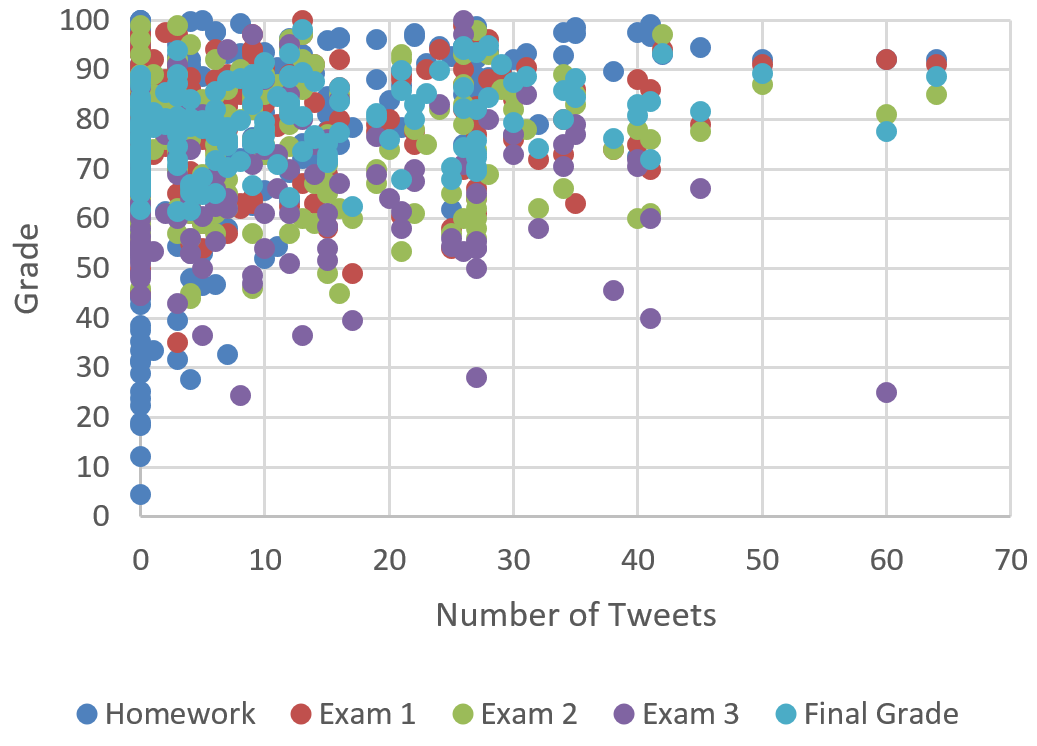
\includegraphics[width=0.75\textwidth]{figures/numTweets.png}
\caption{Homework, exams, and course grades versus number of tweets posted.}
\label{fig:numTweets}
\end{figure}


%------------------------------------------------

\section*{Conclusion}
The use of social media use in the engineering classroom as a means of broadening student engagement with course curriculum was explored through this study. It was demonstrated that performance on traditional course metrics was not influenced by increased participation in the optional or assigned Twitter activities. Further, previous work has found limited little difference on student outcomes measured using concept inventories and course examinations between the cohorts compared on the basis of cohort size \cite{berg_relationship_2015}. It has been the experience of the author that the discussions carried out through Twitter have been meaningful and have extended the learning beyond the walls of the classroom. However, without the motivation of participation being tied to a percentage of the student's course grade, and not in the form of extra credit, these discussions do not occur. 

The Twitter platform has the benefits of enabling real-time communication. Further, students have the opportunity to engage with the online engineering community through communication with practicing engineers that use Twitter. The methods of promoting this both with students and with the engineering community not affiliated with the course remain to be explored.  With the adaptation of tools such as TAGS for automated collection of tweets (including for newly created Twitter accounts), this form of student activity has the potential to promote greater inter-student communication as well as enhance public discourse within the engineering field.


\section*{Acknowledgements}
The author would like to thank the engineering students at the University of Wisconsin-Stout for their photographic and textual contributions.


%----------------------------------------------------------------------------------------
%  REFERENCE LIST
%----------------------------------------------------------------------------------------
\vspace{4\baselineskip}\vspace{-\parskip} % Creaters proper 4 blank line spacing.
\footnotesize % Makes bibliography 10 pt font.
\bibliographystyle{unsrtnat} %Can use a different style as long as it is one which uses numbered references in the text.
\bibliography{refs}

%----------------------------------------------------------------------------------------



\end{document}
